Mathematical models used to simulate water distribution systems are subject to uncertainty. 
Effective characterization of uncertainty is critical for reliable analysis with simulation-based studies. 
Particularly for contamination incidents, uncertainty quantification is needed to effectively 
use simulation tools that provide insights into response actions. 
Hydraulic parameters that might cause uncertainty include: 
(1) customer demands at each node and time, (2) operational controls (e.g., valve settings, pump curves), (3) 
infrastructure topography and characteristics (e.g., missing pipes or junctions, effective pipe diameters) and (4) initial conditions (e.g., tank levels, pump statuses). 
Water quality parameters that might cause uncertainty include: 
(1)  initial water quality, (2) contaminant species, (3) contaminant reaction dynamics, (4) the amount
of contaminant injected, (5) injection location, (6) injection time and (7) injection duration.

The \code{uq} subcommand examines the effect of hydraulic and water quality uncertainty on the extent of contamination in terms of the identification of the contamination source. 
This subcommand can be used to quantify uncertainty after running source identification using the Bayesian probability based formulation (Section \ref{sec.bayesian_algorithm}). Given a particular confidence level, nodes can be categorized according to their probability of contamination. Nodes whose contamination probability, $\gamma_n$, that are above a 
threshold are labeled with respect to their contamination state as LY for ``likely yes,'' LN for``likely no'' and UN for ``unknown.''  
For example, for a 95\% confidence level: 

\[ \left\{ \begin{array}{ll}
         \gamma_n \geq 0.975 & \mbox{LY},\\
        0.025\leq \gamma_n \leq 0.975 & \mbox{UN}, \\
        \gamma_n \leq 0.025 & \mbox{LN} \end{array} \right. 
\] 

With the \code{uq} subcommand 
the effects of uncertainty in customer demand, isolation valve status, bulk reaction rate coefficient and 
contaminant injection location, start time, duration and rate can be studied on the size and location of the contamination incident.

A flowchart representation of the \code{uq} subcommand is shown in Figure \ref{fig:uq_flowchart}. Given a list of EPANET 2.00.12 compatible network models (INP format) 
coupled with a list of injection scenarios (TSG format), the \code{uq} subcommand
runs Monte Carlo simulations to estimate the probability that each node in the network is contaminated.

\begin{figure}[h]
	\centering
	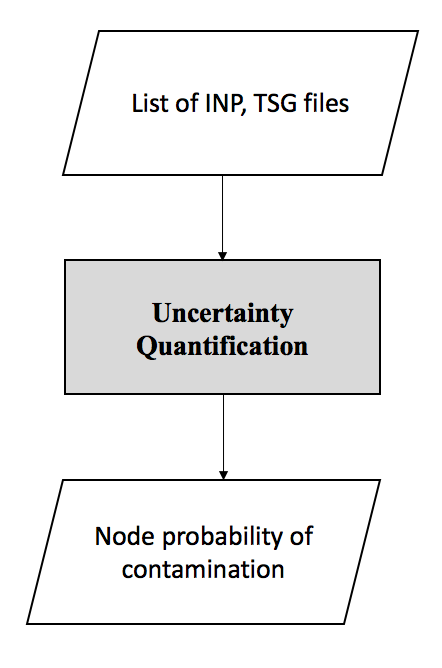
\includegraphics[scale=0.30]{graphics/uq_flowchart.png}
	\caption{Uncertainty quantification flowchart.}
	\label{fig:uq_flowchart}
\end{figure}

\section{Uncertainty Quantification Method}\label{uqn_algorithms}
The \code{uq} subcommand runs an ensemble of scenarios where each scenario is defined using an INP and TSG file. The INP and TSG files 
contain the hydraulic and water quality parameters for the scenario.  
The results are used to compute the probability that each node is contaminated, using the following equation:
\begin{equation}
\gamma_n = \sum_{s \in S} \delta_{s,n}\beta_s
\label{nodeprob}
\end{equation}
where $\gamma_n $ is the probability that node $n$ is contaminated, $\beta_s$ is the probability of scenario $s$ and $\delta_{s,n}$ is a binary parameter that is $1$ if scenario $s$ contaminates node $n$, and $0$ otherwise. The values of $\delta_{s,n}$ are determined from the simulations over the full potential scenario set, and the values for $\beta_s$ are determined using equation~\eqref{source_probability} based on previous measurements provided in the measurements file. If no measurements file is provided, then the values for $\beta_s$ are assumed to be uniform. A threshold value is used to decide whether a node is contaminated or not in a single scenario.

\section{\code{uq} Subcommand}\label{sec.uq_subcommand}

The \code{uq} subcommand is executed using the following command line:
\begin{unknownListing}
wst uq <configfile>
\end{unknownListing}
where \code{configfile} is a WST configuration file in the YAML format.

The \code{---help} option prints information about this subcommand,
such as usage, arguments and a brief description:
\begin{unknownListing}
wst uq --help
\end{unknownListing}

\subsection{Configuration File}

The \code{uq} subcommand generates a template configuration
file using the following command line:

\begin{unknownListing}
wst uq --template <configfile>
\end{unknownListing}

The \code{uq} template configuration file is shown in
Figure \ref{fig:uq_template}. Brief descriptions of the
options are included in the template after the \# sign.

\begin{figure}[h]
  \unknownInputListing{examples/uq_config.yml}{}{1}{17}
  \caption{The \code{uq} configuration template file.}
  \label{fig:uq_template}
\end{figure}

\subsection{Configuration Options}\label{sec.uq_subcommand.config_options}

Full descriptions of the WST configuration options used by the \code{uq} subcommand are listed below.
\begin{description}[topsep=0pt,parsep=0.5em,itemsep=-0.4em]
  \item[{scenario}]\hfill
  \begin{description}[topsep=0pt,parsep=0.5em,itemsep=-0.4em]
    \item[{signals}]\hfill
\\Name of file or directory with information to generate 
                or load signals. If a file is provided the list of inp tsg tuples
                 will be simulated and the information stored in signals files. If
                a directory with the signals files is specified, the signal files will
                be read and loaded in memory. This input is only valid for the uq
                subcommand and the grabsample subcommand with probability based formulations.

                Required input.
  \end{description}
  \item[{uq}]\hfill
  \begin{description}[topsep=0pt,parsep=0.5em,itemsep=-0.4em]
    \item[{analysis time}]\hfill
\\The time at which the manual grab sample should be taken. 
                The algorithm determines the best possible manual grab sample location(s)
                based upon this time. Units: Minutes from the simulation start time in the
                EPANET 2.00.12 INP file.
    \item[{threshold}]\hfill
      \\This threshold determines whether or not an incident impacts a
      location (mg/L).
    \item[{filter scenarios}]\hfill
\\ This options enables filtering scenarios. Only those scenarios 
                that match at least one of the measurements are considered
                in the optimal sampling analysis, default = False.
    \item[{measurement failure}]\hfill
\\The probability that a sensor gives an incorrect reading. Must be between 0 and 1. 
                
                Required input for the Bayesian algorithm, default = 0.05.
    \item[{confidence}]\hfill
\\The probability cut-off value for classifying nodes as certain to be contaminated, 
                uncertain to be contaminated and certain to not be contaminated. The value is 
                between 0 and 1. Nodes with probability greater than (((1-confidence)/2)+confidence) are 
                classified likely to be contaminated or likely yes LY, 
                nodes with probability less than ((1-confidence)/2) are classified likely not contaminated
                LN and nodes with probability in between are uncertain nodes UN.
                
                Required for node classification, default = 0.95 (unitless).
  \end{description}
  \item[{measurements}]\hfill
  \begin{description}[topsep=0pt,parsep=0.5em,itemsep=-0.4em]
    \item[{grab samples}]\hfill
\\The name of the file that contains all the measurements from 
                the manual grab samples and the fixed sensors. The measurement file 
                format is documented in File Formats Section \ref{formats_measFile}.

                Optional input.
  \end{description}
  \item[{configure}]\hfill
  \begin{description}[topsep=0pt,parsep=0.5em,itemsep=-0.4em]
    \item[{output prefix}]\hfill
\\The prefix used for all output files.
                
                Required input.
    \item[{output directory}]\hfill
      \\The output directory to store the results.
    \item[{debug}]\hfill
\\The debugging level (0 or 1) that indicates the amount of debugging 
                information printed to the screen, log file and output yml file. 
                
                Optional input, default = 0 (lowest level).
  \end{description}
\end{description}


\subsection{Subcommand Output}
The \code{uq} subcommand creates two YAML files called <output prefix>\_uq\_scenarios.yml and <output prefix>\_uq\_nodes.yml that contain
a list of probabilities for the scenarios and nodes, respectively.
The log file named <output prefix>uq\_output.log contains basic debugging information. 

\section{Uncertainty Quantification Example}

A list of EPANET 2.00.12 INP and TSG files are required to run the \code{uq} subcommand. The configuration file for this example, uq\_ex1.yml, is shown in Figure \ref{fig:uq_confex1}. 

\begin{figure}[h]
  \unknownInputListing{../../examples/uq_ex1.yml}{}{1}{17}
  \caption{The \code{uq} configuration file for example 1.}
  \label{fig:uq_confex1}
\end{figure}

The file with the list of scenarios for this example is shown in Figure \ref{fig:uq_scenarios}.

\begin{figure}[h]
  \unknownInputListing{../../examples/Net3/uq/list_scenarios.dat}{}{1}{3}
  \caption{List of scenarios.}
  \label{fig:uq_scenarios}
\end{figure}

Summary information is printed to the screen, as shown in Figure \ref{fig:uq_out1}.

\begin{figure}[h]
  \unknownInputListing{examples/uq/uq_ex1_screen_output.txt}{}{1}{31}
  \caption{Screen output for example 1.}
  \label{fig:uq_out1}
\end{figure}

The results from the \code{uq} subcommand can be represented in probability maps using the \code{visualization} subcommand (Chapter 11). 
